%%%%%%%%%%%%%%%%%%%%%%%%%%%%%%%%%%%%%%%%%%%%%%%%%%%%%%%%%%%%%%%%%%%%%%%%%%%%%%%%%%%%%%%%%%%
%%%%%%%%%%%%%%%%%%%%%%%%%%%%%%%%%%%%%%%%%%%%%%%%%%%%%%%%%%%%%%%%%%%%%%%%%%%%%%%%%%%%%%%%%%%
%%%%%%%%%%%%%%%%%%%%%%%%%%%%%%%%%%%%%%%%%%%%%%%%%%%%%%%%%%%%%%%%%%%%%%%%%%%%%%%%%%%%%%%%%%%
%%%%%%%%%%%%%%%%%%%%%%%%%%%%%%%%%%%%%%%%%%%%%%%%%%%%%%%%%%%%%%%%%%%%%%%%%%%%%%%%%%%%%%%%%%%
%%%%%%%%%%%%%%%%%%%%%%%%%%%%%%%%%%%%%%%%%%%%%%%%%%%%%%%%%%%%%%%%%%%%%%%%%%%%%%%%%%%%%%%%%%%
%%%%%%%%%%%%%%%%%%%%%%%%%%.  WRITE YOUR CHAPTER CONTENTS BELOW.  %%%%%%%%%%%%%%%%%%%%%%%%%%
%%%%%%%%%%%%%%%%%%%%%%%%%%%%%%%%%%%%%%%%%%%%%%%%%%%%%%%%%%%%%%%%%%%%%%%%%%%%%%%%%%%%%%%%%%%
%%%%%%%%%%%%%%%%%%%%%%%%%%%%%%%%%%%%%%%%%%%%%%%%%%%%%%%%%%%%%%%%%%%%%%%%%%%%%%%%%%%%%%%%%%%
%%%%%%%%%%%%%%%%%%%%%%%%%%%%%%%%%%%%%%%%%%%%%%%%%%%%%%%%%%%%%%%%%%%%%%%%%%%%%%%%%%%%%%%%%%%

\subsubsection{Introduction}


Computational chemists can support the study of structure-activity relationships in medicinal chemistry by making computer models that can predict the binding affinity of ligands to proteins. Alchemical free energy (AFE) methods are a popular class of methodologies to do so. Some
introductory reading is recommended ~\cite{mey2020best, cournia_allen_sherman_2017, kuhn_firth-clark_tosco_mey_mackey_michel_2020, Hahn2022}.

This tutorial covers the basic principles of alchemical free energy calculations with BioSimSpace; how to setup, simulate, and analyze alchemical Relative Binding Free Energy (RBFE) calculations for congeneric series of protein-ligand complexes; how to set up and analyze alchemical ABFE calculations of a ligand bound to a protein.  
The notebooks prompt the readers to complete a series of exercises that typically involve completing cells to test their understanding of the material presented. 

\subsubsection{Setting up AFE calculations using BioSimSpace}

The first notebook of this tutorial \href{https://github.com/OpenBioSim/biosimspace_tutorials/blob/main/04_fep/01_intro_to_alchemy/alchemical_introduction.ipynb}{alchemical-introduction} introduces the basic functionality available in BioSimSpace to implement AFE calculations. 
The notebook first introduces the functionality of the \href{https://biosimspace.openbiosim.org/api/index_Align.html}{BSS.Align} module. BSS.Align implements a variety of mapping algorithms based on maximum common substructure searches between a supplied pair of molecules to generate a 'merged' molecule used to describe an alchemical transformation. This is used to generate a merged molecule that describes the alchemical transformation of ethane into methanol.
Next, the use of \href{https://biosimspace.openbiosim.org/api/generated/BioSimSpace.Protocol.FreeEnergy.html#BioSimSpace.Protocol.FreeEnergy}{BSS.Protocol.FreeEnergy} is illustrated using the relative hydration free energy of ethanol to methane as an example, using the AFE engines \emph{SOMD} \cite{Calabr2016} or \emph{mdrun}. 
The AFE simulations can in principle be executed directly from the notebook as a set of independent MD simulations run serially, but this is often too slow to be practical. The next section describes protocols to submit calculations in parallel on HPC resources.
Finally, the notebook describes the setup of the relative binding free energy calculation of benzene to o-xylene bound to the protein T4 lyzozyme mutant. 
\\
The notebook then describes the use of \href{https://biosimspace.openbiosim.org/api/generated/BioSimSpace.FreeEnergy.Relative.html#}{BSS.FreeEnergy.Relative} to process the completed AFE simulations for two legs of a thermodynamic cycle using MBAR or TI to obtain a free energy estimate. The resulting free energy changes are subtracted to yield a relative binding free energy for o-xylene to benzene. Finally, the plotting of overlap matrices is demonstrated to assess the reliability of a computed free energy change. The functionality covered by this notebook is illustrated in Figure \ref{thermodynamic_cycle_fig}.

\begin{figure}[htp]
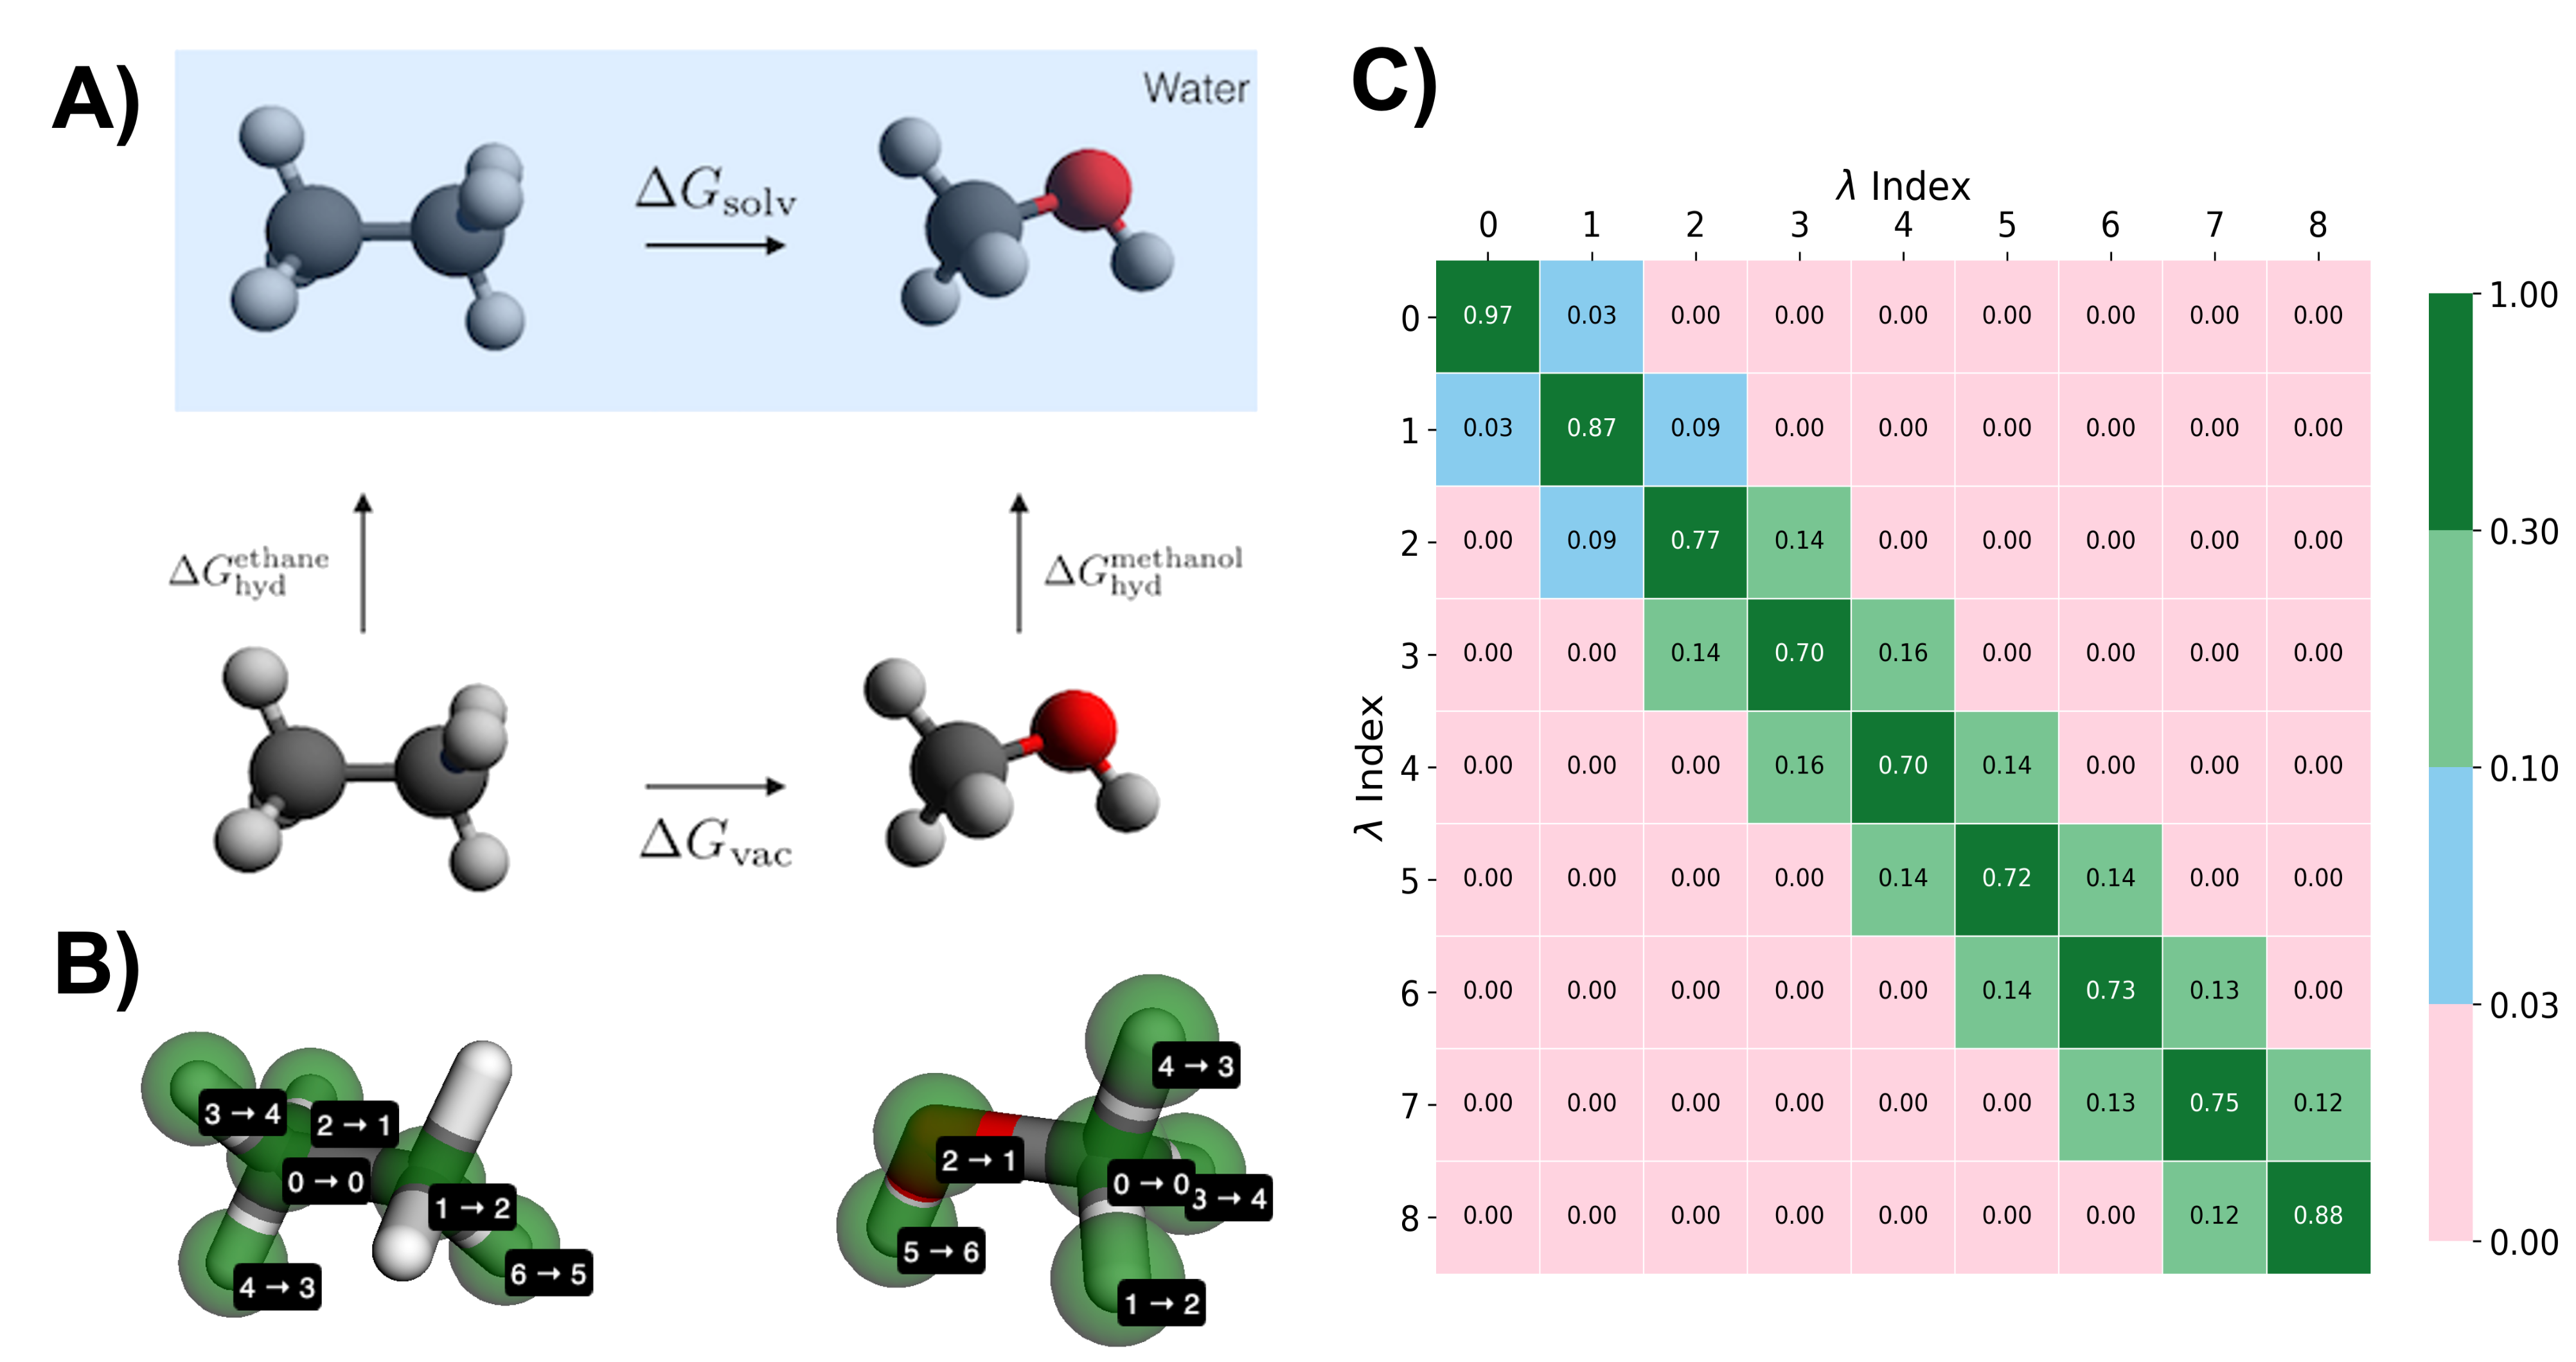
\includegraphics[width=\linewidth]{LIVECOMS/04_fep/introfep_updated.png}
\caption{ \textbf{A)} Thermodynamic cycle used to compute the relative hydration free energy of ethane to methanol. \textbf{B)} Visualisation of the atom mappings between ethane and methanol generated by \emph{BSS.Align}. \textbf{C)} Visualisation of overlap matrix generated by \emph{BSS.Notebook.plotOverlapMatrix} to help assess the reliability of a calculated free energy change.}
\label{thermodynamic_cycle_fig}
\end{figure}


\subsubsection{RBFE calculation pipelines}

The second notebook of this tutorial \href{https://github.com/OpenBioSim/biosimspace_tutorials/blob/main/04_fep/02_RBFE/01_setup_rbfe.ipynb}{01-setup-rbfe.ipynb} shows how to design an RBFE campaign for a congeneric series of protein-ligand complexes. This is illustrated using a dataset of ligands for the protein TYK2, taken from the benchmark set of Wang et al. \cite{Wang2015} 
First, a drop-down menu is presented to the user to enable the selection of a variety of configuration settings (such as the choice of forcefields to use for the ligands, the protein, or the FEP engine to select). In BSS 2023.3.0 the FEP engines \emph{SOMD} and \emph{mdrun} (from the GROMACS software suite) are supported. An \href{https://github.com/michellab/BioSimSpace/tree/feature-amber-fep}{experimental feature branch} that implements support for RBFE calculations with the MD engine pmemd from the AMBER software suite is also available. 

Next, \href{https://biosimspace.openbiosim.org/api/generated/BioSimSpace.Align.generateNetwork.html}{BSS.Align.generateNetwork} is used to interface with the LOMAP software~\cite{Liu2013} to propose a network of relative transformations that span the provided ligand dataset. The notebook illustrates interactive plotting of the proposed network and how to make manual adjustments such as adding or deleting edges or inserting new ligands into the network. Once the user is satisfied with the chosen FEP network, setup instructions are saved to disk. 
\\
Processing the entire TYK2 dataset involves setting up and running several hundred MD simulations of solvated ligands and protein-ligand complexes. This would be impractically slow if executed from a notebook on a single workstation. For convenience, we provide a sample \href{https://github.com/OpenBioSim/biosimspace_tutorials/blob/main/04_fep/02_RBFE/scripts/run_all_slurm.sh}{slurm submission script} that processes the setup, simulation and analysis of the entire network constructed by the RBFE setup notebook on an HPC environment. This script may be adjusted for deployment on different slurm clusters or as reference for the implementation of the execution model on different schedulers. The functionality covered by this notebook is illustrated in Figure \ref{rbfe_setup_fig}.
\\

\begin{figure}[htp]
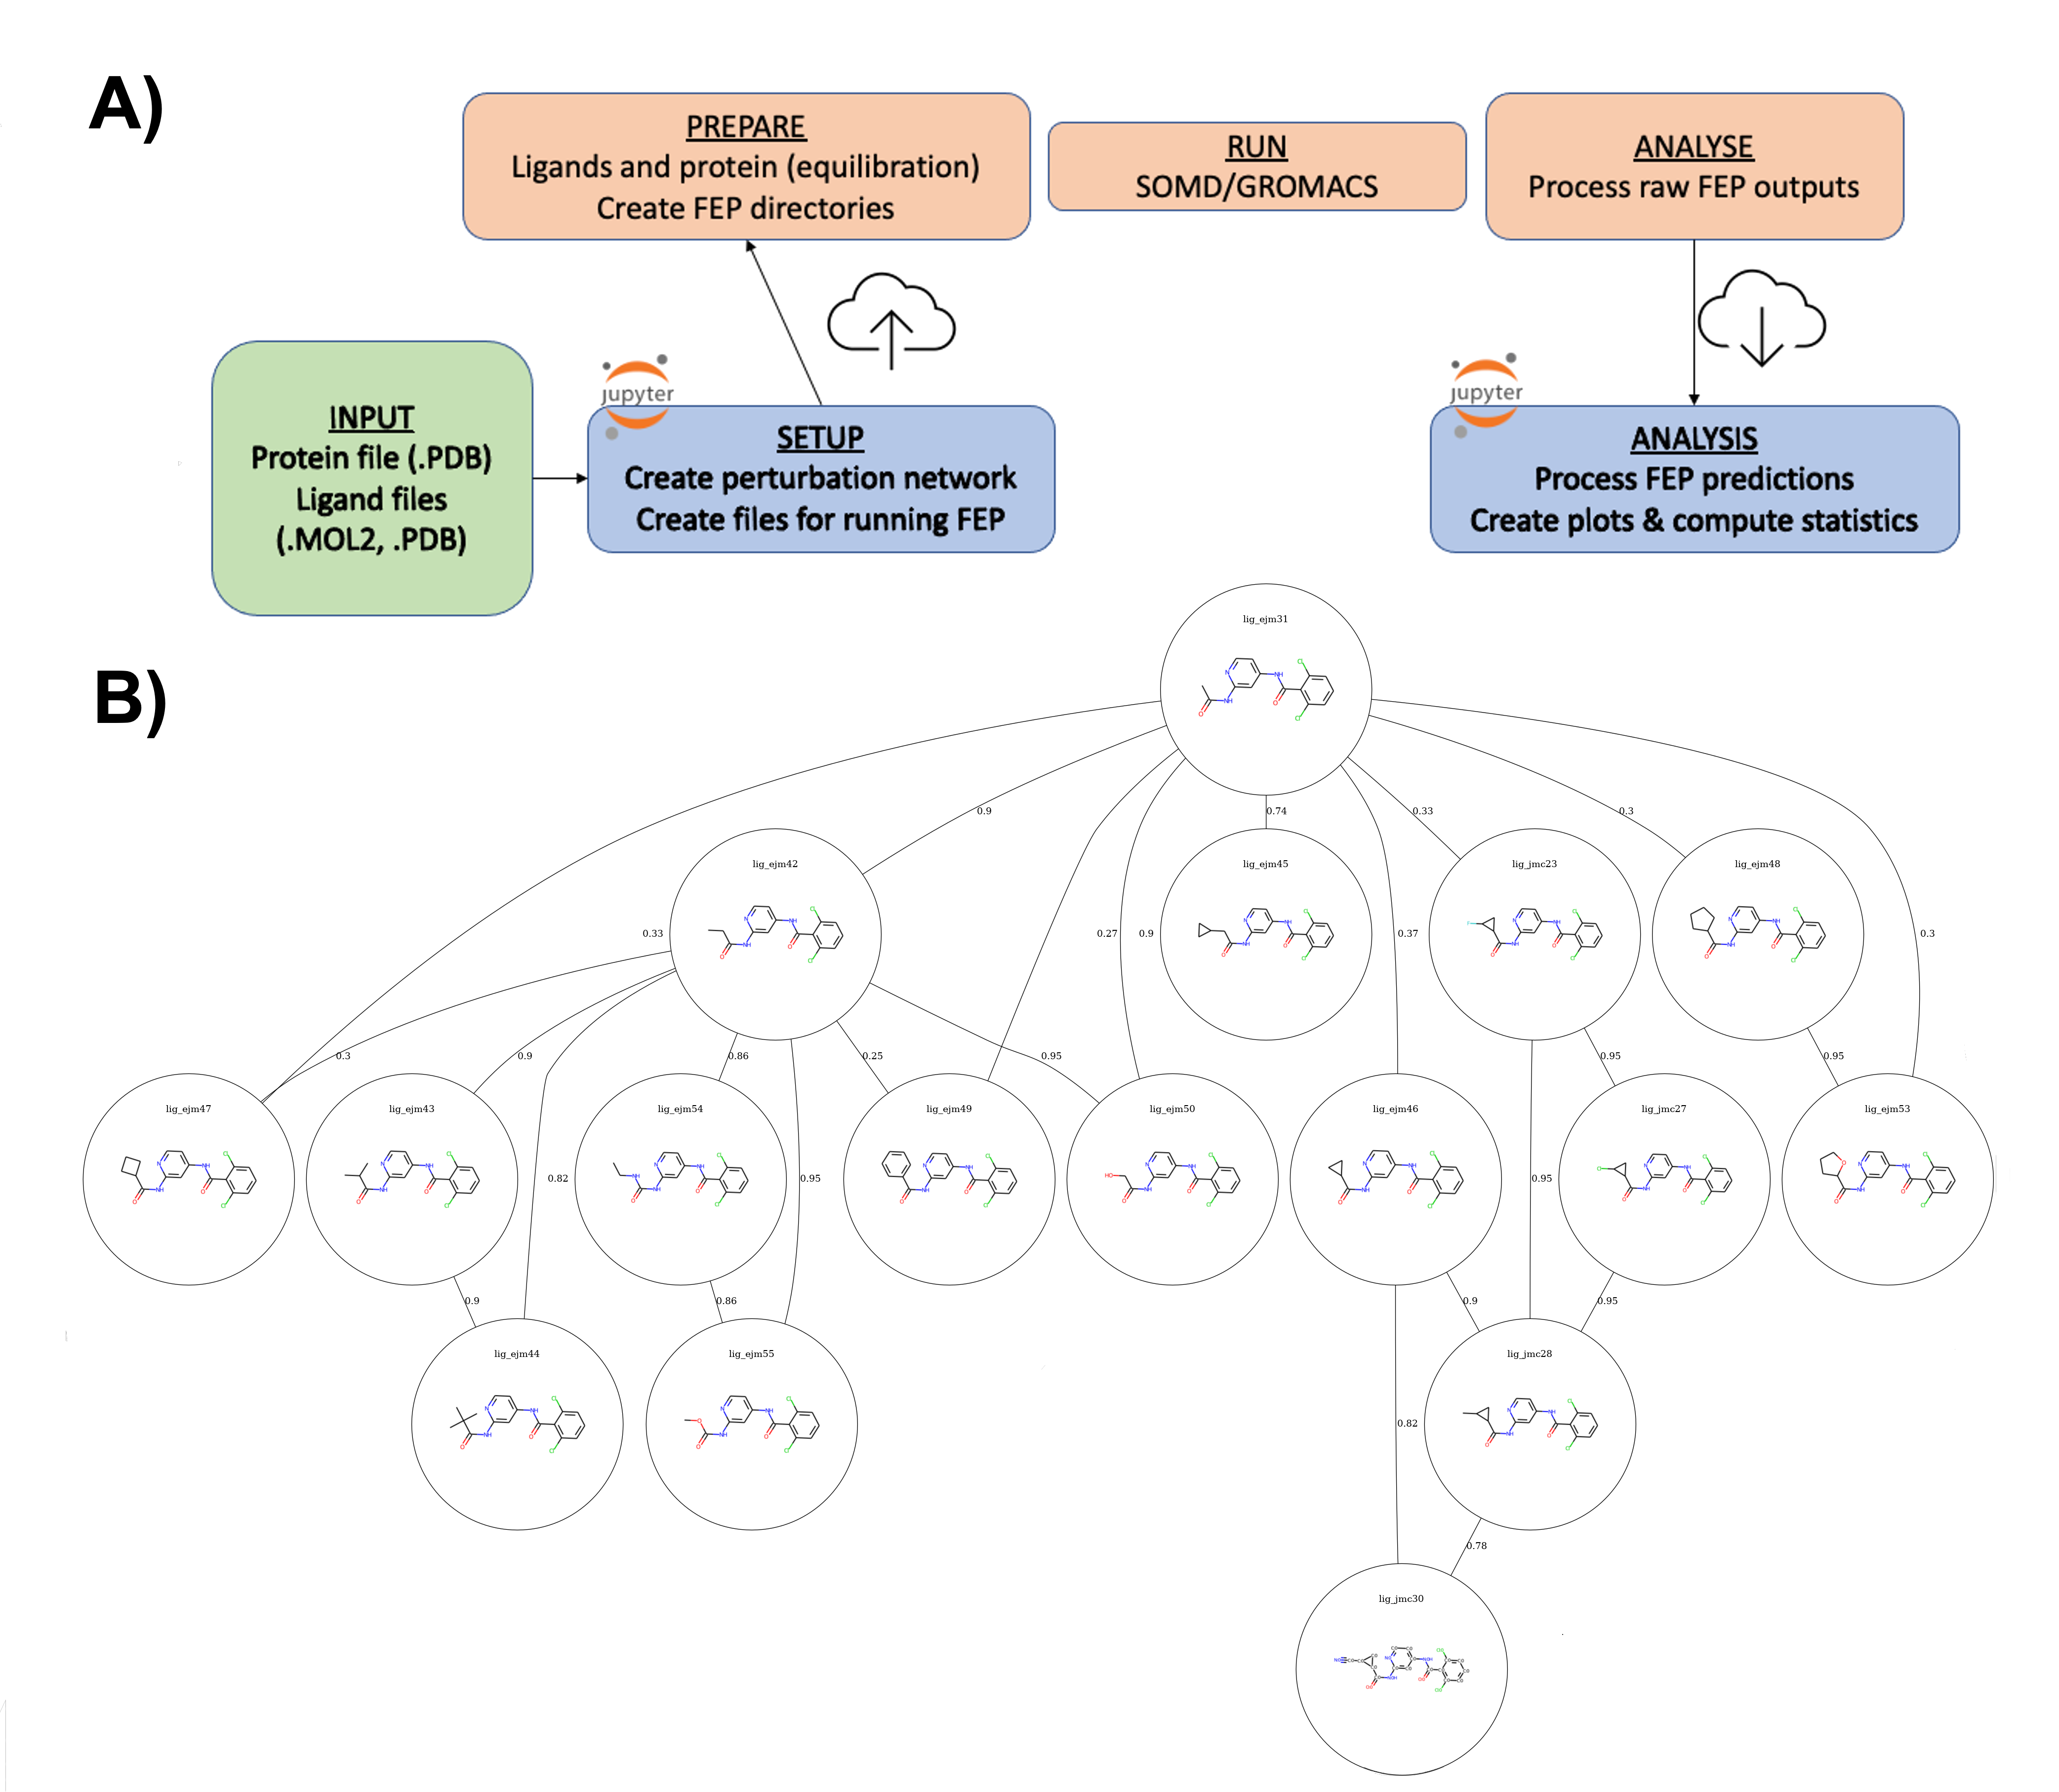
\includegraphics[width=\linewidth]{LIVECOMS/04_fep/rbfe-setup.png}
\caption{ \textbf{A)} Schematic of the RBFE pipeline in this tutorial. Whereas blue boxes represent notebooks run on a local machine, orange boxes represent Python scripts run sequentially on a computing cluster.
\textbf{B)} Perturbation network proposed by \emph{BSS.Align.generateNetwork} for a dataset of TYK2 ligands.} 
\label{rbfe_setup_fig}
\end{figure}


The third notebook \href{https://github.com/OpenBioSim/biosimspace_tutorials/blob/main/04_fep/02_RBFE/02_analysis_rbfe.ipynb}{02-analysis-rbfe} provides a walk-through of the analysis of the processed RBFE network. 
The RBFE network is first visualized using \emph{NetworkX}. Next, mean relative binding free energies are evaluated for each edge by averaging the results from all replicates available for each edge. The standard error of the mean is used as an estimate of the statistical uncertainty of each edge RBFE. A scatter plot comparing relative vs calculated binding free energies is produced, this is only possible because experimental data is available for this dataset. 
\\
Next, the set of RBFEs is converted into a set of binding free energies with an arbitrary reference value using the \emph{cinnabar} software to produce a scatter plot of calculated vs experimental binding free energies, together with statistical measures of accuracy (mean unsigned error, root mean squared error, Pearson coefficient, and Kendall tau coefficient). The functionality covered by this notebook is illustrated in Figure \ref{rbfe_analysis_fig}.
\\

\begin{figure}[htp]
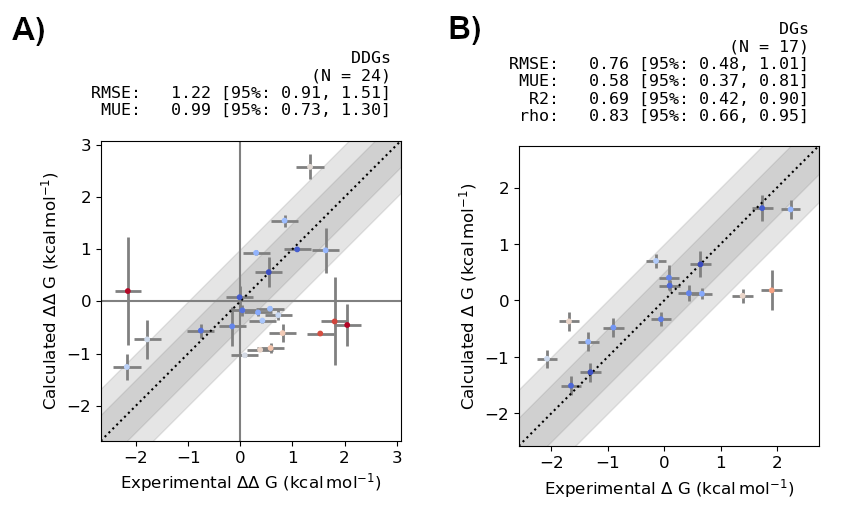
\includegraphics[width=\linewidth]{LIVECOMS/04_fep/rbfe-analysis.png}
\caption{ \textbf{A)} Scatter plot of experimental vs computed pairwise $\Delta \Delta G_{bind}$ free energies from the analysed perturbation network. \textbf{B)} Scatter plot of $\Delta G_{bind}$ estimates after processing of the network. } 
\label{rbfe_analysis_fig}
\end{figure}

\subsubsection{ABFE calculations}
%
The fourth notebook \href{https://github.com/OpenBioSim/biosimspace_tutorials/blob/main/04_fep/03_ABFE/01_setup_abfe.ipynb}{01-setup-abfe} describes how to set up alchemical ABFE calculations with BSS for use with either \emph{mdrun} or \emph{SOMD}. This free energy functionality is currently implemented in Exscientia's sandpit area of this version of BioSimSpace. Sandpits are used to test experimental features without accidentally breaking core functionality of the toolkit. 

Although RBFE calculations can be very useful in drug discovery, several important problems lie outside the scope of standard RBFE calculations. These include the calculation of the binding free energies of structurally dissimilar ligands to a common target; the calculation of the binding free energies of the same ligand to the same protein with different binding poses; the calculation of the binding free energies of a single ligand to a range of targets, as would be required to optimize selectivity or promiscuity. These quantities can be calculated using alchemical ABFE calculations because they utilize a more general \emph{double decoupling} thermodynamic cycle than in RBFE calculations \cite{gilson_statistical-thermodynamic_1997}. This involves entirely removing the ligand's intermolecular interactions in the presence of restraints between the ligand and receptor, as shown in Figure \ref{abfe_fig}A. 

\begin{figure}[htp]
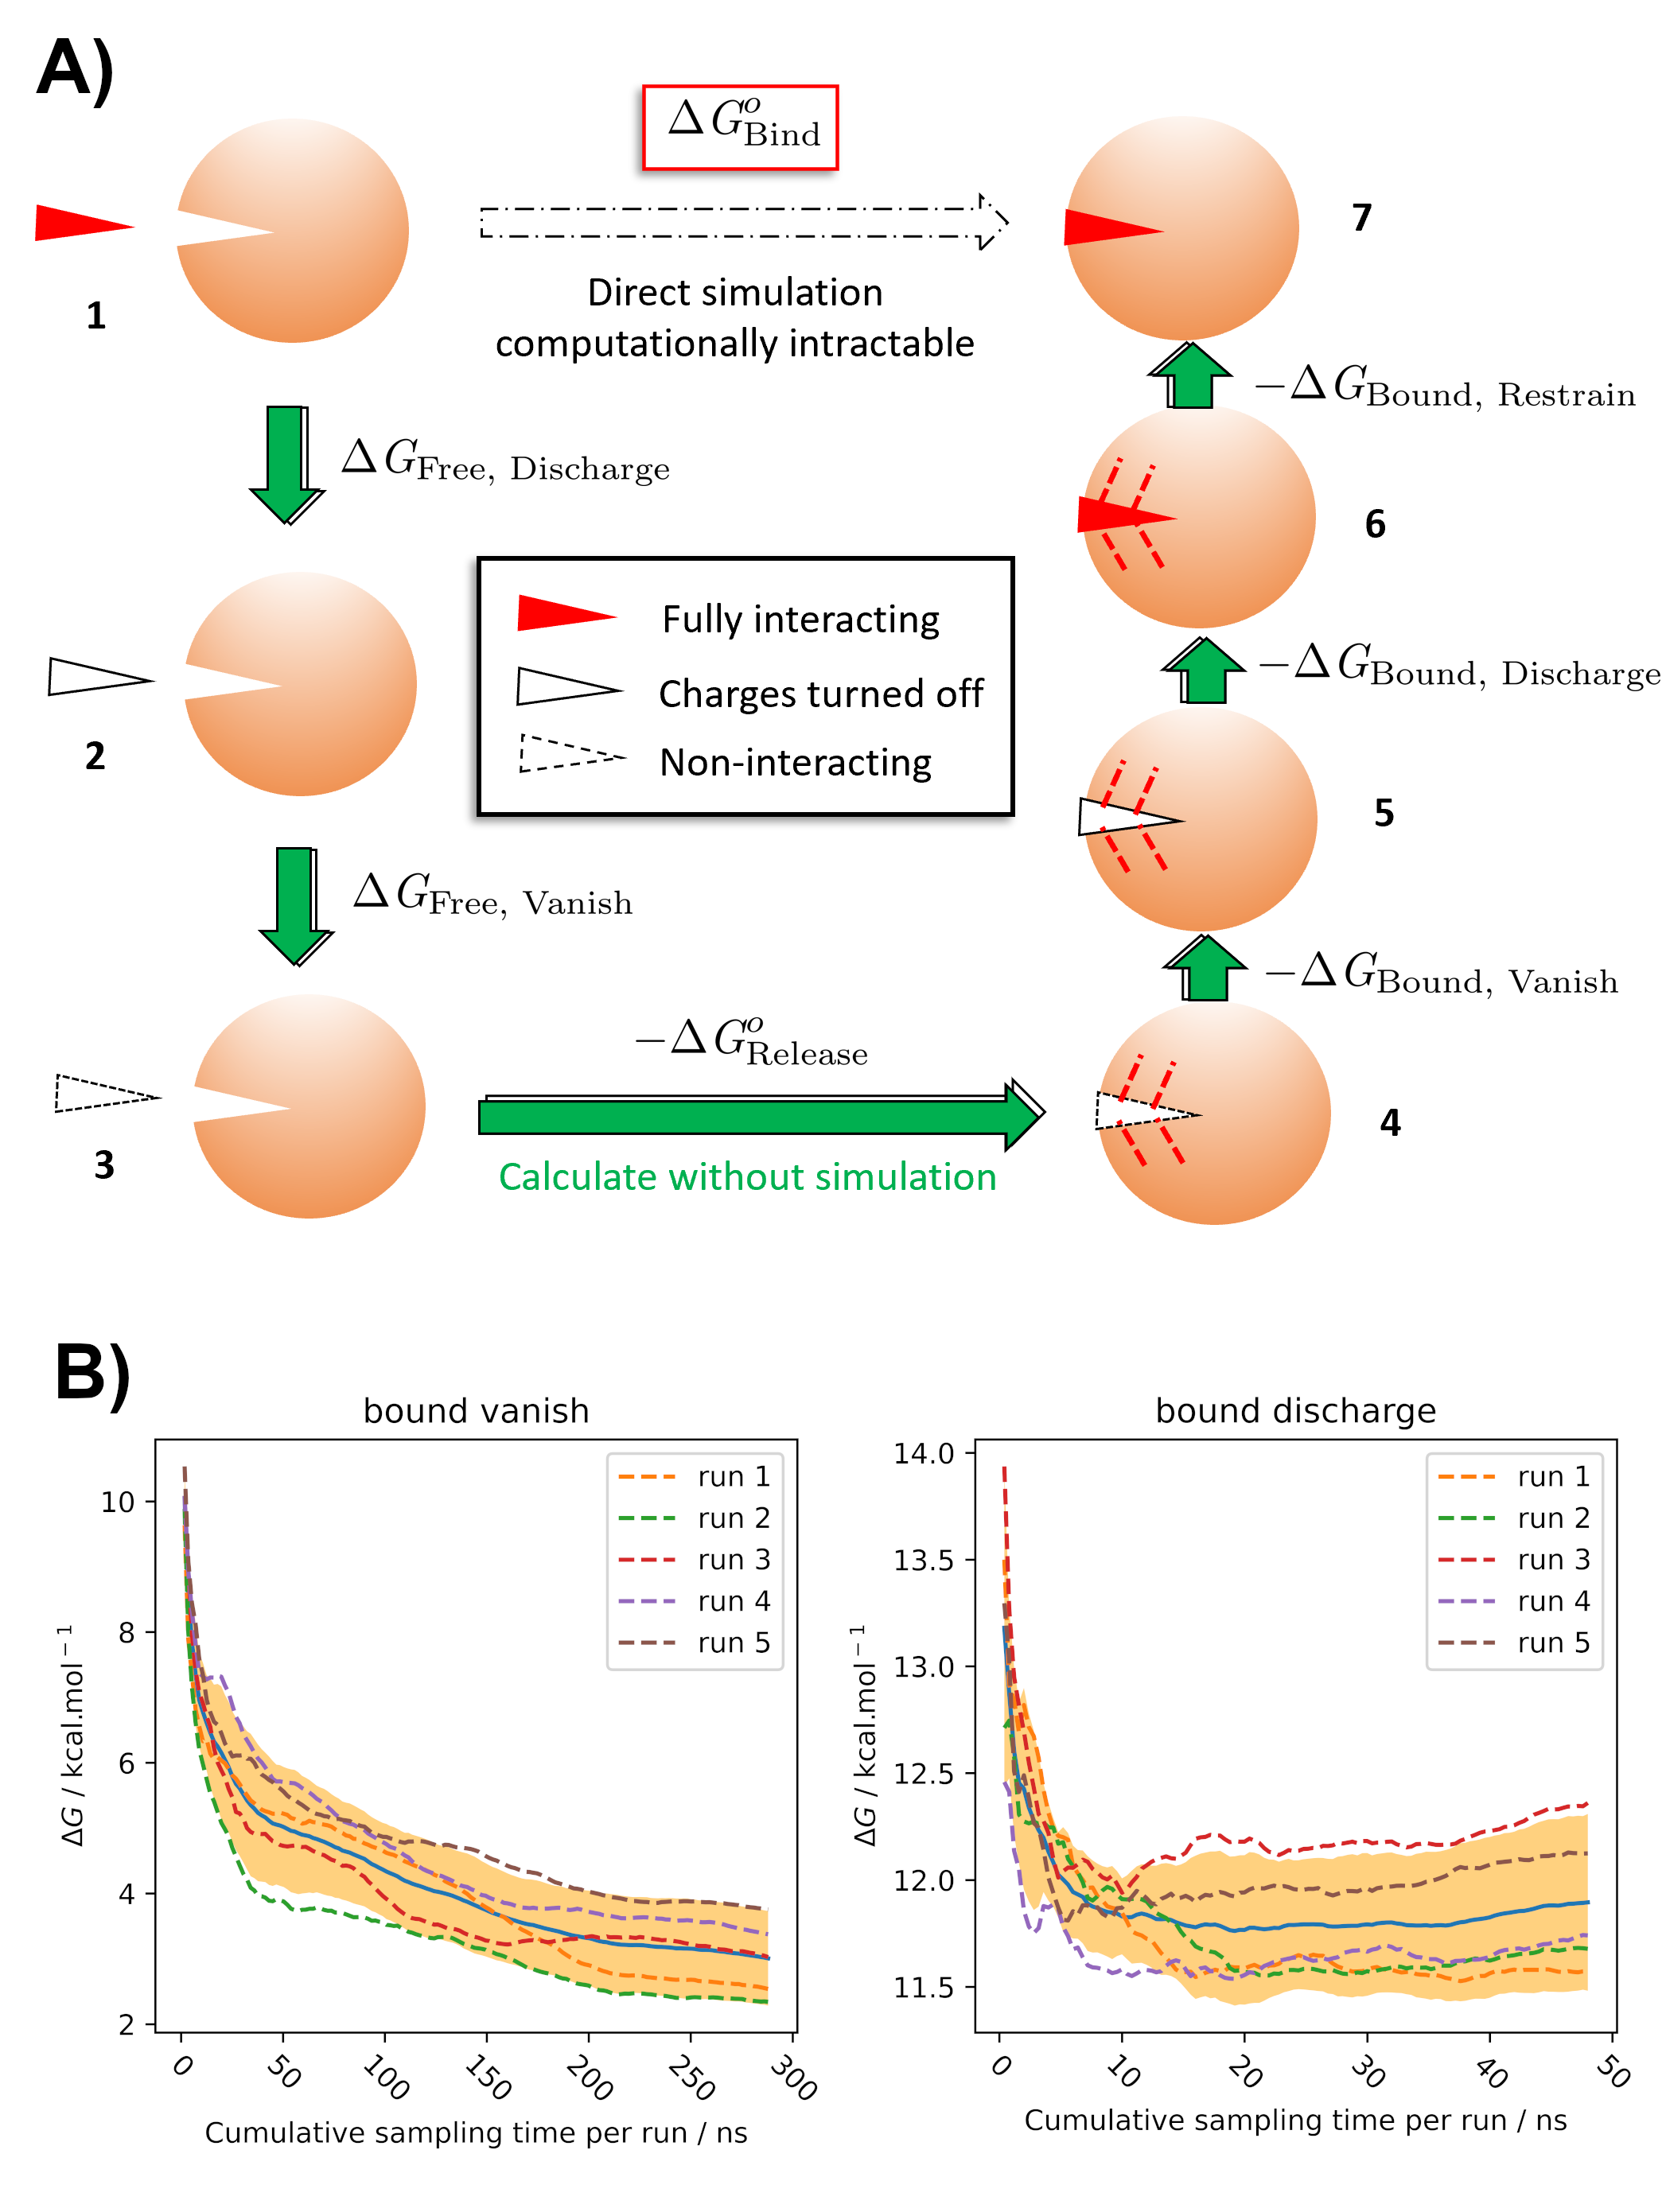
\includegraphics[width=\linewidth]{LIVECOMS/04_fep/abfe-tutorial.png}
\caption{ \textbf{A)} Thermodynamic cycle for alchemical absolute binding free energy calculations. \textbf{B)} Sample convergence plots for legs 5 and 6 of the ABFE thermodynamic cycle for the MIF/MIF180 complex, showing especially poor convergence for the bound vanish stage prior to discarding initial non-equilibrated samples.} 
\label{abfe_fig}
\end{figure}

The notebook describes the use of \textit{BSS.Align.decouple} to tag a molecule in a BSS system that should have all its intermolecular interactions removed to compute its absolute binding free energy. This is illustrated here with the use of the ligand MIF180 bound to the protein MIF \cite{Qian2019, Clark2023}. 

Next, it is shown how to run and analyse a simulation of the fully-interacting protein-ligand complex to generate the required intermolecular restraints. Both actions are handled using \textit{BSS.FreeEnergy.RestraintSearch}. The popular 6-degrees of freedom Boresch restraints are supported \cite{boresch_absolute_2003}, as well as a Clark's multiple distance restraints (MDR) methodology \cite{Clark2023}.
The notebook illustrates the automated generation of Boresch or MDR restraints with BSS. The algorithm implemented aims to select stable restraints which mimic strong native receptor-ligand interactions. The notebook includes visualization of the chosen restraints before free energy inputs are prepared, which allows the user to identify cases where the selected restraints may not be optimal, or where symmetry corrections may be required \cite{duboue-dijon_building_2021}. The notebook then demonstrates the use of \textit{BSS.FreeEnergy.AlchemicalFreeEnergy} to generate input files for the engines SOMD or GROMACS. This class in the Exscientia sandpit contains all of the functionality from \textit{BSS.FreeEnergy.Relative} in the main version of the code, as well as additional functionality required for ABFE calculations.

Since ABFE calculations can be time-consuming we recommend parallel execution of the different legs of the thermodynamic cycle using an approach similar to that used in the RBFE tutorial.
\\

The fifth notebook \href{https://github.com/OpenBioSim/biosimspace_tutorials/blob/main/04_fep/03_ABFE/02_analysis_abfe.ipynb}{02-analysis-abfe} describes how to analyse an ABFE calculation to estimate the free energy of binding of a ligand. Sample output simulation data are provided for each leg of the double decoupling thermodynamic cycle and analysed using \textit{BSS.FreeEnergy.AlchemicalFreeEnergy.Analyse} to plot potentials of mean forces. The standard free energy of binding is then obtained by summing the free energy changes from each leg and adding a standard state correction term for the use of Boresch restraints, along with any symmetry corrections required. The notebook also describes how to carry out convergence analyses (see Figure \ref{abfe_fig}B) to assess the robustness of the ABFE estimates.  
